\section{Data Compression}
Before we can talk about data compression it is necessary to explore the meaning and the functiong of encodings. Given two alphabets $A={a_1,a_2,\ldots,a_k}$ and $B={b_1,b_2,\ldots,b_k}$ an encoding is function:
\begin{equation}
    \varphi: A^* \longrightarrow B^*
\end{equation}
For a function to be a suitable encoding it must be at least an injective function (one-way function). In information theory and in data encoding in particular we refer to injective encoding as \textbf{uniquely decodable} encodings.
Prefix codes are uniquely decodable codes that can be decoded without delay and are written in the form:
\begin{equation}
    A=\{a_1, a_2, \ldots, a_k\} \xrightarrow{\varphi} B=\{b_1, b_2, \ldots, b_D\}
\end{equation}
where $\varphi_i = |\varphi(a_i)|$
    \subsection{Kraft-McMillen 1958 Inverse Theorem}
    If $\varphi$ is a uniquely decodable code, then:
    \begin{equation}
        \sum_{i=1}^{k}{D^{-l_i}}<=1
    \end{equation}
    $D$ is the cardinality of the output alphabet, $l_i$ is the lenght of the encoding for $a_i$. We can quickly see that, there can't be an uniquely decodable code that uses three encodings of length 1 to map over the binary alphabet:
    \begin{equation}
        A=\{a,b,c\},\quad B=\{0,1\}, \quad
        l_a=l_b=l_c=1 \longrightarrow \frac{1}{2}+\frac{1}{2}+\frac{1}{2} >1
    \end{equation}
    Instead, if we were to insist on using a length 10 encoding for everyone of the input characters:
    \begin{equation}
        A=\{a,b,c\},\quad B=\{0,1\},\quad
        l_a=l_b=l_c=10 \longrightarrow \frac{1}{2^{10}}+\frac{1}{2^{10}}+\frac{1}{2^{10}} << 1
    \end{equation}
    \subsubsection{Proof 1}
    Assume the code is uniquely decodable and it is a prefix code, we can sort the input alphabet so that the length of the encoding satisfies the following:
    $$a_1\leq a_2\leq\ldots\leq a_k$$
    A character with an enconding of length $i$ generates a sub-tree rooted in $a_i$ with height $l-l_i$. This sub-tree contains $D^(l-l_i)$ nodes that cannot be used in the encoding because they would share an encoded prefix.\\
    Insert diagram\\
    In the original three the following number of leaves  $$D^l - \sum_{i=1}^{k-1}{D^{l-l_1}}$$
    The $k-1$ term that bounds the sum is needed because we need to make sure that one last leaf is available to assign it to the last character $a_k$.
    \begin{equation}
        \setlength{\jot}{10pt}
        \begin{WithArrows}
        D^l-\sum_{i=1}^{k-1}{D^{l-l_i}} &\geq 1 \Arrow[xoffset=1cm]{Group by $D^l$} \\
        D^l(1-\sum_{i=1}^{k-1}{D^{-l_i}}) &\geq 1 \Arrow[xoffset=1cm]{Divide by $D^l$} \\
        1-\sum_{i=1}^{k-1}{D^{-l_i}}\geq &D^{-l} \Arrow[xoffset=1cm]{$D^{-l}$ is the last term of the sum}\\
        1 \geq \sum_{i=1}^{k}{D^{-l_i}}&
        \end{WithArrows}
        \nonumber
    \end{equation}
    \subsubsection{Proof 2 - General case}
    Let's define $N(n,h)$ the number of strings of alphabet $A^n$ having encoding length h. It must be true that $N(n,h)\leq D^h$ because $\varphi$ is uniquely decodable.
    \begin{equation}
        D^{-l_1}+D^{-l_2}+\ldots+D^{-l_k}\leq 1 \\
    \end{equation}
    $\forall n, n\in\mathbb{N}$ let's consider the object $(D^{-l_1}+D^{-l_2}+\ldots+D^{-l_k})^n$. If written as a product it takes the following form:
    $$D^{-l_1\cdot n}+D^{-l_1\cdot(n-1)-l_2}+\ldots+D^{-l_k\cdot n}$$
    As $n$ tends towards infinity the exponent will behave differently depending on the value of the base. If the base is $<1$ it will be bound between 0 and 1, and in any case $<1$. If the base is $>1$ it will grow towards infinity faster than any polynomial function. Lastly, if the base is $=1$ it will remain constant. To prove the theorem we will demonstrate that the object is dominated by a linear function, meaning that it cannot be in the second case. 
    All of the members' exponents follow this chain of disequalities: $l_1\cdot n\leq exp\leq l_k\cdot n$. That is, because we sorted the character by encoding length, 1 being the shortest while $k$ the longest.
    \begin{align*}
        \underset{prob. 0}{N(n,1)}D^{-1}+\ldots+N(n,l_1\cdot n)D^{l_1\cdot n}+\ldots+N(n,l_k\cdot n)D^{-l_k\cdot n}\\\leq D^1D^{-1}+\ldots+D^{l_k}D^{-l_k} \leq l_k\cdot n
    \end{align*}
    Since the object is dominated by $l_k\cdot n$ which is linear, it must mean that it also grows at most linearly, meaning that the base of the exponent must be $\leq 1$.
    \subsection{Kraft-McMillen Direct Theorem}
    If given $l_1,l_2,\ldots,l_k$ and $D$ such that $\sum_{i=1}^{k}{D^{-l_i}}\leq 1$ there must exist a prefix code $\varphi$ having $l_1,l_2,\ldots,l_k$ as lengths of the encoding.
    \subsubsection{Proof}
    Proof can be given by construction by producing the complete D-ary tree \\
    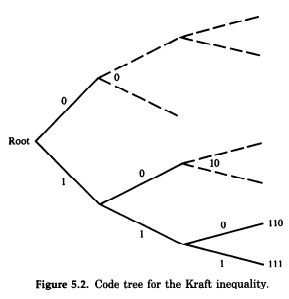
\includegraphics[width=8cm]{Information Theory/Data Compression/Kraft-McMillen-Inequality-Proof-Diagram.png}\\
    \textbf{Observation:} Prefix codes compress as good as any other uniquely decodable code.
    \subsubsection{Average expected code length - Definition}
    Given the input alphabet A, P the probability and B the output we define the Expected Length as:
    \begin{equation}
        EL(\varphi)=\sum_{i=1}^{k}{p_i\cdot l_i}=\sum_{i=1}^{k}{p_i|\varphi(a_i)|}
    \end{equation}
    Our goal is to find prefix codes that minimize $EL$.
    
    \subsection{1st Shannon Theorem 1948}
    If $\varphi$ is uniquely decodable code then $EL(\varphi)\geq \mathcal{H}_D(P)=\sum_{i=1}^{k}{p_i\cdot log_D{p_i}}$
    The proof relies on Kraft-McMillen theorem and this simple logarithmic property:
    $$log_e{x}\leq x-1, \quad -log_e{x}\geq 1-x$$
    \subsubsection{Proof}
    \hspace*{-2cm}
    \begin{align*}
        \setlength{\jot}{10pt}
        \begin{WithArrows}
        &EL(\varphi)-\mathcal{H}_D(P) = \sum_{i=1}^k{p_i\cdot l_i}+\sum_{i=1}^{k}{p_i\cdot log_D{p_i}} \Arrow[xoffset=1cm]{Group by $p_i$ and force $l_i$ as $log_D$} \\
        &=\sum_{i=1}^{k}{p_i\cdot log_D{(D^{l_i}p_i)}} \Arrow[xoffset=-2cm]{Change to base e, take out the common term}\\
        &=\frac{1}{log_e{D}}\cdot \sum_{i=1}^{k}{p_i\cdot log_e{(D^{l_i}p_i)}} \Arrow[xoffset=-2cm]{Group by $-1$}\\
        &=\frac{-1}{log_e{D}}\cdot \sum_{i=1}^{k}{p_i\cdot log_e{\frac{1}{D^{l_i}p_i}}} \Arrow[xoffset=-2cm]{Using the above property}\\
        &\geq \frac{-1}{log_e{D}}\cdot \sum_{i=1}^{k}{p_i\cdot (\frac{1}{D^{l_i}p_i}}-1) \\
        &= \frac{-1}{log_e{D}}\cdot \bigg{(}\sum_{i=1}^{k}{\frac{1}{D^{l_i}}} - \underset{=1}{\cancel{\sum_{i=1}^{k}{p_i}}} \bigg{)} \Arrow[xoffset=-1.5cm]{Group by $-1$}\\
        &=\frac{1}{log_e{D}}\bigg{(}\underset{KMM\longrightarrow \geq 0}{1-\sum_{i=1}^{k}{\frac{1}{D^{l_i}}}} \bigg{)}\geq 0
        \end{WithArrows}
    \end{align*}
    An optimum code achieves the equality between the expected lenght and the entropy of the distribution.
    \subsection{Shannon Code}
    Let's recall the definition of expected lenght and entropy over the probability P and alphabet with cardinality D:
    $$EL(\varphi) = \sum_{i=1}^{k}{p_i\cdot l_i}$$
    $$ \mathcal{H}_D(P) = \sum_{i=1}^{k}{p_i\cdot (-\log_{D}{p_i})}$$
    Observation: $\log_{D}{\frac{1}{p_i}} \in \mathbb{R},\quad l_i \in \mathbb{N} \longrightarrow l_i=\lceil\log_{D}{\frac{1}{p_i}}\rceil$\\
    If $\sum_{i=1}^{k}{D^{-l_i}} \leq 1$ then we can use the Direct Theorem to prove $\varphi$, with encoding lenghts $l_1, l_2, \ldots l_k$, exists. The encoding is obtained with a greedy strategy on the D-ary tree: \
    $$\sum_{i=1}^{k}{D^{-l_i}} =\sum_{i=1}^{k}{D^{-\lceil \log_{D}{\frac{1}{p_i}} \rceil}}\leq 1$$
    $$ \lceil{\log_{D}{\frac{1}{p_i}}}\rceil = \log_{D}{\frac{1}{p_i}}+\beta_i \quad 0 \leq \beta_i < 1$$
    $$\sum_{i=1}^{k}{D^{\log_{D}{p_i-\beta_i}}} = \sum_{i=1}^{k}{D^{\log_{D}{p_i}}\cdot \frac{1}{D^{\beta_i}}} = \sum_{i=1}^{k}{p_i\cdot \underset{\geq 1}{\frac{1}{D^{\beta_i}}}} \leq 1$$
    Example: 
    $A = \left\{ a, b \right\}  B=\left\{ 0,1 \right\}$
    $ P=\left\{ 1-\frac{1}{32}, \frac{1}{32} \right\}$
    $l_b = \log_2{2^5} = 5$ $\lceil \log_2{1-\frac{1}{32}}\rceil = 1 = l_a$
    But this is not efficient because we are assigning unnecessarily long codes to characters with low probability.
    \subsubsection{Sub-Optimality of Shannon Codes}
    We can demonstrate that Shannon Codes are suboptimal:
    \begin{align*}
        EL(S) &= \sum_{i=1}^{k}{p_i (-\log{p_i}+\beta_i)}\\
        &=\sum_{i=1}^{k}{p_i (-\log{p_i})} + \sum_{i=1}^{k}{p_i \beta_i}\\
        &=\mathcal{H}_D(P) + \sum_{i=1}^{k}{p_i\beta_i}\leq \mathcal{H}_D(P)+1 \quad \sum_{i=1}^{k}{p_i\cdot\beta_i} \leq1
    \end{align*}
    $$\mathcal{H}_D(P) \leq EL(\varphi) \leq \mathcal{H}_D(P)+1$$
    



    %%%%%%%%%%%%%%%%%%%%%%%%%%%%%%%%%%%%%%%%%%%%%%%%%%%%
    \subsection{Shannon-Fano Code}
    Given the alphabet A with characters $a_1, a_2, \ldots, a_k $ mapping to the probabilities $ p_1\leq p_2\ldots \leq p_k$. The aim is to balance the sum of the probabilities assigned to the branches of the root. To obtain balance we try to minimize this absolute value: $|\sum_{i=1}^{h}{p_i}- \sum_{i=h+1}^{k}{p_i}|$. We then repeat the calculation recursively.\\
    Example: 
    $$A= \left\{ a,b,c,d,e,f \right\}$$
    $$\quad P=\left\{ \underbrace{\frac{40}{100}, \frac{18}{100}}_{\frac{58}{100}}, \underbrace{\frac{15}{100}, \frac{13}{100}, \frac{10}{100}, \frac{4}{100}}_{\frac{42}{100}} \right\}$$
    \begin{figure}[htbp]
        \centering
        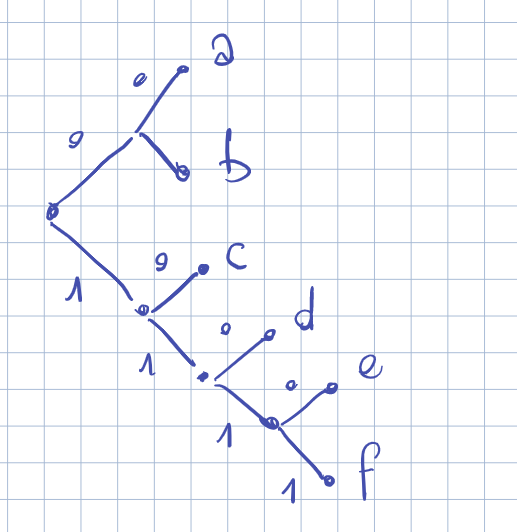
\includegraphics[width = 6cm]{Information Theory/Data Compression/ShannonFano-Tree.png}
    \end{figure}\\
    Shannon-Fano is compromising on splitting the characters set in two of equal (or best possible) probability because the problem of splitting a set in equally weighted subsets is NP-Complete.\newline



    %%%%%%%%%%%%%%%%%%%%%%%%%%%%%%%%%%%%%%
    \subsection{Shannon on strings of lenght n over input alphabet}
    Example: $A=\left\{ a,b \right\} \;B=\left\{ 0,1 \right\}\; P=\left\{ \frac{3}{4}, \frac{1}{4} \right\}\; \mathcal{H}_2(P)=0.81\;$ 
    $EL(\varphi) = 1.25$\\
    Let's define the efficiency of a code as follows:
    $$Eff. = \frac{\mathcal{H}_D(P)}{EL(\varphi)}\leq 1$$
    Applying to our example we get: 
    $$Eff. = \frac{\mathcal{H}_2(P)}{EL(\varphi)}=0.64$$
    Let's try to calculate the efficiency now with an encoding for pairs of characters:
    $$A'=\left\{ aa, ab,ba,bb \right\}\; P'=\left\{ \frac{9}{16}, \frac{3}{16}, \frac{3}{16}, \frac{1}{16} \right\} = P^2 \;$$ $$
    \mathcal{H}_D(P')= 1.62 = \mathcal{H}_D(P^2) = 2\cdot \mathcal{H}_D(P)$$
    $$EL(\varphi) = 1.93 Eff. = 0.83$$
    If we pretend we want to send a message 1000 characters long, with the single character encoding we expect a message lenght of 1.25k characters,
    Instead with the pairs encoding we expect $\frac{1.93}{2} \leadsto 0.97k \;$characters.\\\\
    \textbf{Property}: given two events x, y independent
    $\mathcal{H}(x \wedge y) = H(x) + H(y)$
    Proof:
    \begin{align*}
        H(x \wedge y ) &= -\sum_{i,j}^{}{p_i \cdot q_j \log{(p_i\cdot q_j)}} = - \sum_{i,j}^{}{p_i \cdot q_j \log{p_i}} - \sum_{i,j}^{}{p_i\cdot q_j \log{q_j}}\\
        &= -\underset{=1}{\sum_{j}{q_j}} \cdot \sum_{i}^{}{p_i \log{p_i}} - \underset{=1}{\sum_{i}{p_i}} \cdot \sum_{j}{q_j \log{q_j}} = \mathcal{H}(x) + \mathcal{H}(y)
    \end{align*}
    From Shannon Theorem we then have $EL(\varphi_n) \geq \mathcal{H}_D(P^n) = n\cdot \mathcal{H}_D(P)$\\
    For Shannon Codes (and all sub-optimal codes) we have:
    $$ n\cdot \mathcal{H}_D(P) \leq EL(\varphi_n) < n\cdot \mathcal{H}_D(P)+1$$ If we want to reason in terms of a single input alphabet value
    we divide the disequality by n. We can see that for $n \leadsto \infty $ the expected lenght is squeezed between the terms of the disequality.



    %%%%%%%%%%%%%%%%%%%%%%%%%%%%%%%%%%%%%%%%%%%%%%%%%%%
    \subsection{Huffman Codes}
    Given the input alphabet and the probability distribution
    $A = \left\{ a_1, a_2, \ldots, a_k \right\} \; P={p_1\leq p_2 \ldots \leq p_k}$
    We start by taking the two leasts probable characters and we put them at the leaves, creating a phantom character with probability
    the sum of the two. I keep repeating this process until we obtain a complete tree.

    \subsection{History}
    \begin{itemize}
        \item 1949 Shannon-Fano code
        \item 1952 Huffman code
        \item 1970 Huffman becomes popular
        \item 1977 Lempel and Ziv create the LZ77 Code (Variable length - Block)
        Uses a dynamic dictionary for compression.
        \item 1978 They update it with a new version LZ78 with static dictionary
        Gets patented by Sperry Corporation $\rightarrow$ Unisys 1981
        \item 1983 Another variant LZW (W - Welch) is a simpler implementation of LZ78. In the same year they request a patent and publish an article in 1984 withouth mentionign its patent.
        \item 1985 the patent gets actually officialized
        \item Unix and Compuserve start using the code
        \item 24/12/1994 Unisys decides to claim the royalties "The GIF Tax"
        \item 2004 the patent expires
        \item Unix decides to avoid the taxation by "downgrading" to LZ77
    \end{itemize}
    
    \subsection{LZ-77}
    The idea is to focus on a part of the message i've already codified and i refer to it as search buffer.
    The portion just in front of the search buffer is the look-ahead buffer. The lenght of both buffers is a parameter of the implementation.
    I then operate like this: I look for the longest prefix of the look-ahead buffer that also appears as a substring in the search buffer.
    In reality it's a little more complex as the substring from the search buffer can overflow in the look-ahead buffer.
    Let's identify as j the position occupied by the first character of the substring and i the position of the first character of the prefix.
    We then consider the triple (o, l, s): 
    \begin{itemize}
        \item o: distance between i and j
        \item l: length of the prefix-suffix
        \item s: the first mis-matching character
    \end{itemize}
    \subsection{Example}
    $input = babbababbabbabba $ Buffer size: 5\\
    Encoding:
    \begin{description}
        \item[1st step] S buffer = $\emptyset$, LA buffer = babba, triple = (0,0,b)
        \item[2nd step] S buffer = b, LA buffer: abbab, triple (0,0,a)
        \item[3rd step] S buffer: ba, LA-buffer = bbaba, triple= (2,1,b)
        \item[4th step] S buffer: babb, LA-buffer = ababb, triple = (3,2,a)
        \item[5th step] S buffer: bbaba la-buffer = bbabb, triple = (5,4,b)
        \item[6th step] S buffer:bbabb la-buffer= abba, triple= (3,4,@)
    \end{description}
    Decoding:
    \begin{description}
        \item[1st step] @@@@@b
        \item[2nd step] @@@@@ba
        \item[3rd step] @@@@@babb
        \item[4th step] @@@@@babbaba
        \item[5th step] @@@@@babbababbabb
        \item[6th step] @@@@@babbababbabbabba
    \end{description}
    

    